%% %%%%%%%%%%%%%%%%%%%%%%%%%%%%%%%%%%%%%%%%%%%%%%%%%
%% Template for a conference paper, prepared for the
%% Food and Resource Economics Department - IFAS
%% UNIVERSITY OF FLORIDA
%% %%%%%%%%%%%%%%%%%%%%%%%%%%%%%%%%%%%%%%%%%%%%%%%%%
%% Version 1.0 // November 2019
%% %%%%%%%%%%%%%%%%%%%%%%%%%%%%%%%%%%%%%%%%%%%%%%%%%
%% Ariel Soto-Caro
%%  - asotocaro@ufl.edu
%%  - arielsotocaro@gmail.com
%% %%%%%%%%%%%%%%%%%%%%%%%%%%%%%%%%%%%%%%%%%%%%%%%%%
\documentclass[11pt]{article}
\usepackage{UF_FRED_paper_style}
\usepackage{fancyhdr}

\usepackage{lipsum}  %% Package to create dummy text (comment or erase before start)

\usepackage{listings}
\usepackage{listings-golang}
\usepackage{color}


%% ===============================================
%% Setting the line spacing (3 options: only pick one)
% \doublespacing
% \singlespacing
\onehalfspacing
%% ===============================================

\setlength{\droptitle}{-5em} %% Don't touch

\setlength{\parindent}{0pt}

% %%%%%%%%%%%%%%%%%%%%%%%%%%%%%%%%%%%%%%%%%%%%%%%%%%%%%%%%%%
% SET THE TITLE
% %%%%%%%%%%%%%%%%%%%%%%%%%%%%%%%%%%%%%%%%%%%%%%%%%%%%%%%%%%

% TITLE:
\title{TSA Covid Finance}


\pagestyle{fancy}
\fancyhf{}
\rhead{\today}
\lhead{Anna Huber \& Joshua Hemmings}
\rfoot{\thepage}

% AUTHORS:
%\author{Anna Huber% Name author
% \and Joshua Hemmings %% Email author 2
%    }
    
% DATE:
%\date{\today}

% %%%%%%%%%%%%%%%%%%%%%%%%%%%%%%%%%%%%%%%%%%%%%%%%%%%%%%%%%%
% %%%%%%%%%%%%%%%%%%%%%%%%%%%%%%%%%%%%%%%%%%%%%%%%%%%%%%%%%%
\begin{document}
% %%%%%%%%%%%%%%%%%%%%%%%%%%%%%%%%%%%%%%%%%%%%%%%%%%%%%%%%%%
% %%%%%%%%%%%%%%%%%%%%%%%%%%%%%%%%%%%%%%%%%%%%%%%%%%%%%%%%%%
% ABSTRACT
% %%%%%%%%%%%%%%%%%%%%%%%%%%%%%%%%%%%%%%%%%%%%%%%%%%%%%%%%%%
% %%%%%%%%%%%%%%%%%%%%%%%%%%%%%%%%%%%%%%%%%%%%%%%%%%%%%%%%%%
%{
%\maketitle
%}
\begin{center}
\textbf{\Large TSA Covid Finance}    
\end{center}

% %%%%%%%%%%%%%%%%%%%%%%%%%%%%%%%%%%%%%%%%%%%%%%%%%%%%%%%%%%
% %%%%%%%%%%%%%%%%%%%%%%%%%%%%%%%%%%%%%%%%%%%%%%%%%%%%%%%%%%
% BODY OF THE DOCUMENT
% %%%%%%%%%%%%%%%%%%%%%%%%%%%%%%%%%%%%%%%%%%%%%%%%%%%%%%%%%%
% %%%%%%%%%%%%%%%%%%%%%%%%%%%%%%%%%%%%%%%%%%%%%%%%%%%%%%%%%%

% --------------------
\section{Introduction}
% --------------------
COVID-19 currently dictates our lives and is one topic which is highly discussed. It is proven, that more people have died during this pandemic than usual (\cite{owidcoronavirus}). In this short paper we want to analyse the affect of COVID-19 on the major financial markets of following five countries: Switzerland, Germany, Italy, United States and China.

% --------------------
\section{Literature Review}
% --------------------
The author of the "Stock markets reaction to COVID-19: Cases or fatalities?" article (\cite{stock-covid-reaction}) has discovered that the stock markets responded negatively to the increase of confirmed COVID-19 cases. An increase in confirmed COVID-19 cases affects stock markets in a light manner. During the beginning of the pandemic stock markets have reacted strongly due to uncertainty.



% --------------------
\section{Methods}
% --------------------
In order to investigate a causality between the corona case numbers and financial market data, the first step is to prepare the data so that they are comparable with each other. After cleansing and preparing the data, the "Augmented Dickey-Fuller Test" is used to check whether the time series are stationary. If the time series are not stationary, the time series are modified using the \lstinline{diff(log())} method (). This procedure is repeated until the "Dickey-Fuller Test" shows that the time series are stationary. Then, the stationary time series are used for the calculation of vector autoreggressive models (VAR models). Furthermore, Granger causality tests are performed.

\subsection{Descriptive Analysis: Visualization, data preparation and decomposition of time series}

\begin{figure}[!htb]
\centering
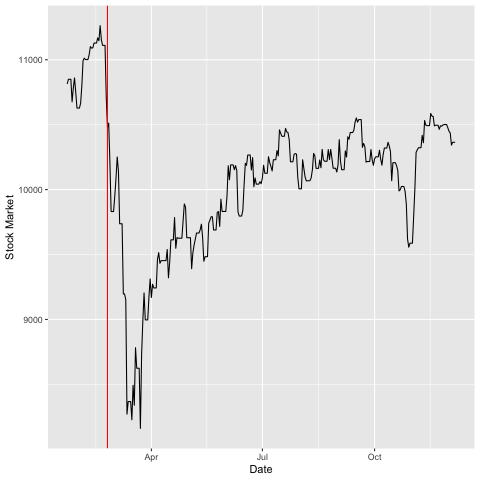
\includegraphics[width=100mm]{R-Code/plots/switzerlandFinance.png} \\
\caption{USA stock market and first confirmed COVID-19 case}
\end{figure}




\subsubsection{Datapreparation: Returns}
In the financial sector, in addition to the absolute level of a time series, its growth rates/returns are often of interest.
Since continuous growth rates/returns are additive due to logarithmizing and more closely match the normal distribution, they are often preferred to discrete returns in time series analysis and econometrics in general. (\cite{PowerPoi49:online})
$$r_{t} =\ln \left(Y_{t}\right)-\ln \left(Y_{t-1}\right)$$

\subsection{Stationarity}
In order to create the VAR models, we must first ensure that the time series are stationary. "A stationary time series is one whose statistical properties such as mean, variance, autocorrelation, etc. are all constant over time."(\cite{Stationa72:online}) For verification, the Augemented Dicky Fullman test is performed on all time series. The test returns the following p-values for the corona case numbers per country:
\begin{table}[h!]
\centering
\caption{P-Values }
\label{tab:p-values-corona}
\begin{tabular}{|l|l|}
\hline
\textbf{Country} & \textbf{P-Value} \\ \hline
China            & 0.01             \\ \hline
Italy            & 0.01             \\ \hline
Switzerland      & 0.99             \\ \hline
Germany          & 0.24             \\ \hline
USA              & 0.99             \\ \hline
\end{tabular}
\end{table}
For the time series of Switzerland, USA and Germany the P-value is greater than 0.05, meaning these time series are not stationary. Therefore we try to create stationarity by using the first differences. Since the $log(0)$ is not defined, we only use the \lstinline{diff()} function and  not the \lstinline{diff(log())} function.
\begin{table}[h!]
\centering
\caption{P-Values after first Differences}
\label{tab:p-values-first-diff}
\begin{tabular}{|l|l|}
\hline
\textbf{Country} & \textbf{P-Value} \\ \hline
Switzerland      & 0.03             \\ \hline
Germany          & 0.02             \\ \hline
USA              & 0.15             \\ \hline
\end{tabular}
\end{table}

\begin{table}[h!]
\centering
\caption{P-Values after second Differences}
\label{tab:p-values-second-diff}
\begin{tabular}{|l|l|}
\hline
\textbf{Country} & \textbf{P-Value} \\ \hline
USA              & 0.99             \\ \hline
\end{tabular}
\end{table}

\subsection{VAR-Modell and Granger Causality}

$$
\begin{array}{l}
Y_{t}=a_{1}+\beta_{11} Y_{t-1}+\beta_{12} X_{t-1}+\beta_{13} Z_{t-1}+\epsilon_{1, t} \\
X_{t}=a_{2}+\beta_{21} X_{t-1}+\beta_{22} Y_{t-1}++\beta_{23} Z_{t-1}\epsilon_{2, t}\\
Z_{t}=a_{1}+\beta_{31} Z_{t-1}+\beta_{32} X_{t-1}++\beta_{33} Y_{t-1}\epsilon_{3, t}
\end{array}
$$
% --------------------
\section{Results}
% --------------------
% --------------------
\subsection{Outlook}
% --------------------



\section{Appendix}


\begin{figure}[h!]
\centering
  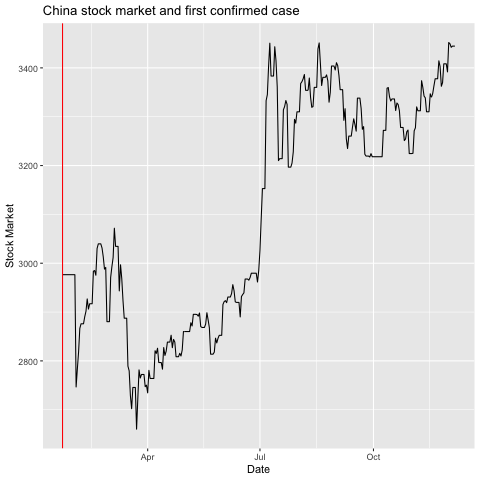
\includegraphics[width=100mm]{R-Code/plots/chinaFinance.png} 
  \caption{China stock market and first confirmed COVID-19 case}
\end{figure}

\begin{figure}[!h]
\centering
  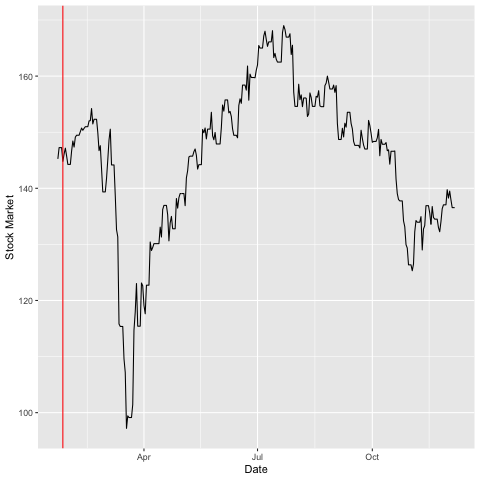
\includegraphics[width=100mm]{R-Code/plots/germanyFinance.png}   
  \caption{Germany stock market and first confirmed COVID-19 case}
\end{figure}

\begin{figure}[!h]
\centering
  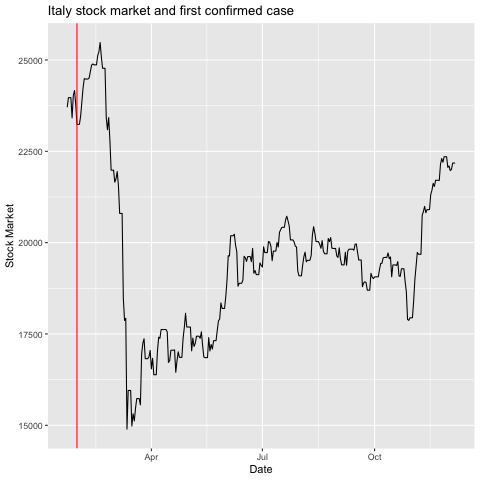
\includegraphics[width=100mm]{R-Code/plots/italyFinance.png}  
  \caption{Italy stock market and first confirmed COVID-19 case}
\end{figure}

\begin{figure}[!h]
\centering
  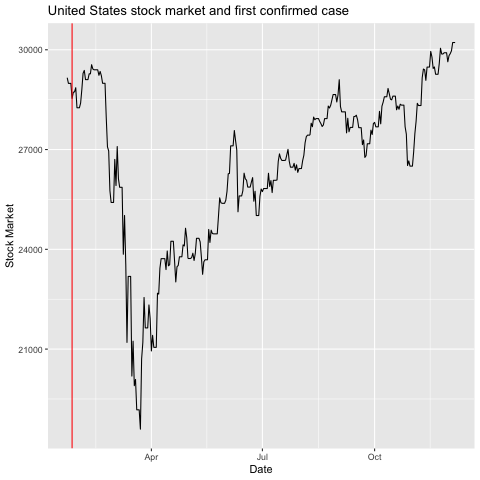
\includegraphics[width=100mm]{R-Code/plots/usaFinance.png} 
    \caption{USA stock market and first confirmed COVID-19 case}
\end{figure}

% %%%%%%%%%%%%%%%%%%%%%%%%%%%%%%%%%%%%%%%%%%%%%%%%%%%%%%%%%%
% %%%%%%%%%%%%%%%%%%%%%%%%%%%%%%%%%%%%%%%%%%%%%%%%%%%%%%%%%%
% REFERENCES SECTION
% %%%%%%%%%%%%%%%%%%%%%%%%%%%%%%%%%%%%%%%%%%%%%%%%%%%%%%%%%%
% %%%%%%%%%%%%%%%%%%%%%%%%%%%%%%%%%%%%%%%%%%%%%%%%%%%%%%%%%%
\clearpage
\medskip
\newpage
\bibliography{references.bib} 

\end{document}